
%%%%%%%%%%%%%%%%% Introduction to the Assignment %%%

In this Assignment, \textit{\textbf{Problem 3 - Propagation Effects \& Targets}}, ...


%%%%%%%%%%%%%%%%% TASK 1 %%%
\section{Radar Performance}

\subsection{Phenomena affecting radar performance}
\label{chap:diffraction}
The performance of a radar is affected by couple of different phenomena, which degrade or attenuate the sent and received signal.
\begin{enumerate}
	\item \textbf{Atmospheric attenuation} \newline
			Atmospheric attenuation is a major loss term, since the radar beam is attenuated as it's travelling through the atmosphere and its constituents (2-way-loss).
			Water vapor, e.g. clouds, rain or fog, and its density as well as temperature are playing a major role in attenuating the signal. This attenuation is also frequency dependant, e.g. higher frequencies are more attenuated, c.f. fig \ref{fig:attenuation}.
			\begin{figure}[!htbp]
			\centering
			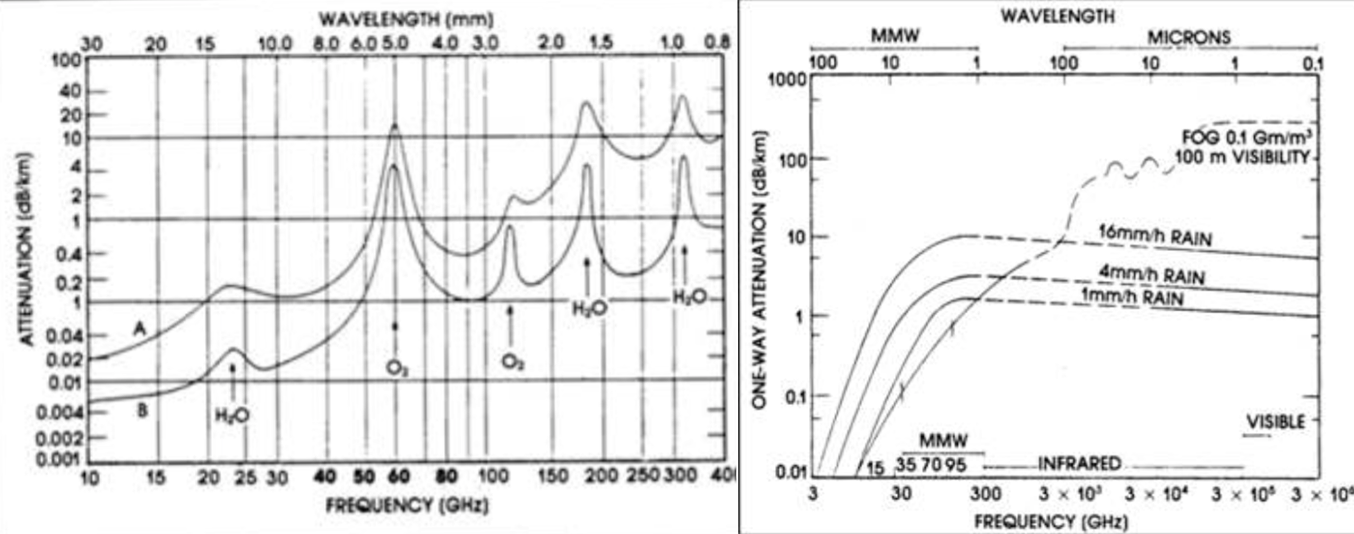
\includegraphics[width=0.9\textwidth]{images/attenuation}
			\caption{atmospheric attenuation as function of frequency \citep{erickson:lecture}}
			\label{fig:attenuation}
			\end{figure}
	\item \textbf{Surface reflection} \newline
			Surface reflection, the reflection of an EM-wave off earth's surface, can lead to multi-path effects when the receiver is hit by the reflected EM-wave, thus leading to measurements that do not correspond with the direction of the original radar beam (assuming an atmospheric radar).
	\item \textbf{Diffraction} \newline
			Diffraction describes the process, when an EM-wave hits an obstacle and is bend around its corners, thus the EM-wave can illuminate things even in a so-called \textit{"shadow zone"}, the zone behind an obstacle. In radar terms, this particular effect can be used to extend the range even beyond the horizon for lower frequencies, since for higher frequencies the diffraction is not very effective.
	\item \textbf{Refraction} \newline
			Atmospheric Refraction is the "bending" of an EM-wave as it propagates through the atmosphere. Refraction is dependant on the constituent of the penetrated material, but also on the thickness of the material and the wavelength of the beam, since the refractive index changes with frequency (optical dispersion) \citep{erickson:lecture}.
	
\end{enumerate}



\subsection{22 GHz and 60 GHz Operation}
Radar is seldom used at 22GHz or 60GHz since at these frequencies the atmosphere is vastly attenuating the signal. Components responsible for the absorption in case of 22GHz is Oxygen ($O_2$) and at 60GHz water vapour ($H_2O$), c.f. fig. \ref{fig:absorb}.
\begin{figure}[h!]
	\centering
	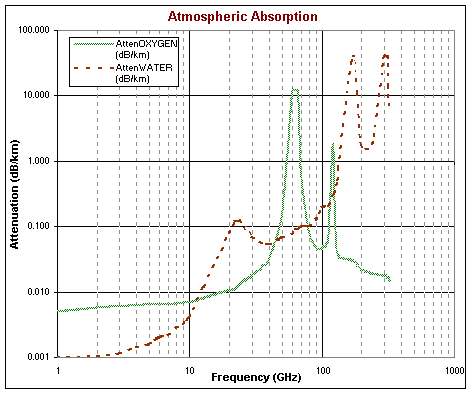
\includegraphics[width=0.7\linewidth]{images/absorbtion}
	\caption{Atmospheric attenuation of different frequencies \protect\footnotemark}	
	\label{fig:absorb}
\end{figure}
\footnotetext{source: \href{http://www.rfcafe.com/references/electrical/images/atm_absorption.gif}{RFCafe}}



%%%%%%%%%%%%%%%%% TASK 2 %%%
\section{Radar cross section (RCS)}

\subsection{Behaviour of normalized RCS}
Figure \ref{fig:RCS} shows the normalized Radar Cross Section of a sphere as function of its circumference in wavelength. The relative RCS is increasing, until the wavelength $\lambda$ equals the circumference, then starts to oscillate until the wavelength is about $\frac{1}{10}$ of the circumference, where the RCS is equal to the normalized RCS, and frequency independent. The first region, the increasing relative RCS, is also called the Rayleigh region, and the latter one the Optical region.\\
The highly fluctuating and oscillation region (Mie) occurs due to interferences of the front face specular return and due to the surface creeping waves, that propagate around the back of the sphere (c.f. chap. \ref{chap:diffraction}) \citep{richards2010principles}.

\begin{figure}[h!]
	\centering
	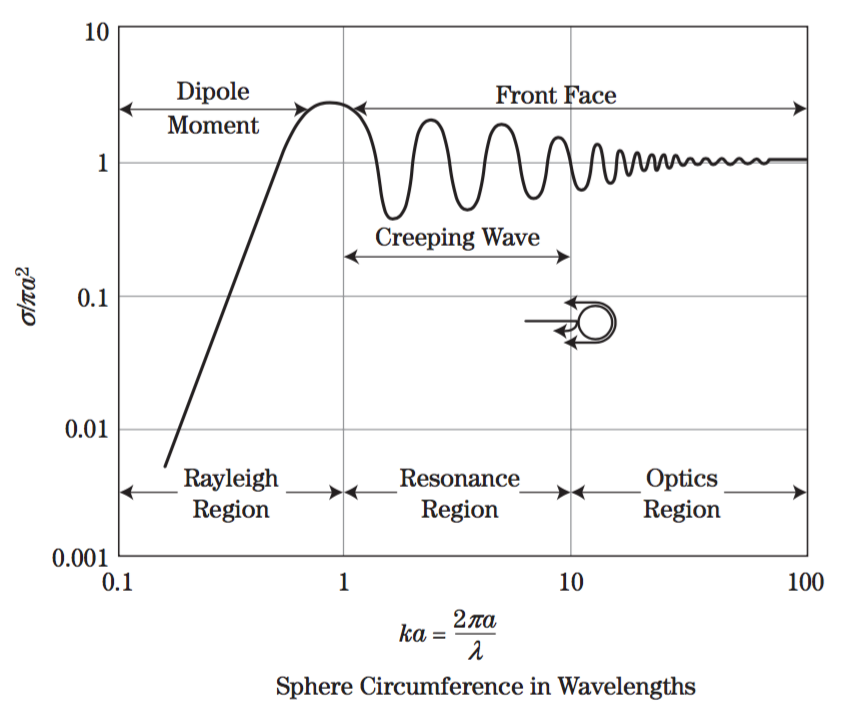
\includegraphics[width=0.8\textwidth]{images/nRCS}
	\caption{Scattering in different regions	 (\citep[c.f.][Fig. 6-12]{richards2010principles})}
	\label{fig:RCS}
\end{figure}

\subsection{Low specular RCS}
A low specular RCS means, that the target is hardly visible to a radar that is illuminating the target. According to Richards et al. \citep{richards2010principles}, one must take into account up to three differenct mechanisms:
\begin{itemize}
	\item Minimize the physical cross section of the target, to minimize the EM wave energy intercepted
	\item Use of \textit{Radar Absorbing Materials} (RAM) to absorb as much of the EM wave as possible, to reduce the amount of reflected energy towards the radar receiver.
	\item Design the shape and surface such as the least amount of energy reflected is reflected towards the radar receiver
\end{itemize}


%%%%%%%%%%%%%%%%% TASK 3 %%%
\section{Radar parameters affecting performance}

\subsection{Surface clutter}
\label{sec:surfaceClutter}


\begin{itemize}
	\item \textbf{Pulse width}\newline
		If the returned signal is covered or limited by surface clutter, one could increase the pulse width to increase the energy that is sent out, thus increasing the energy reflected by the target and therefore increasing the SNR at the receiver \citep{richards2010principles}.
		In contrary, shortening the pulse worsens the SNR at the receiver but improves the unambiguous range.		
	\item \textbf{Antenna gain} \newline
		Increasing or Decreasing the antenna gain increases, respectively decreases the received power, but since the surface clutter is included in the received signal, the surface clutter is also affected by the antenna gain, thus decreasing or increasing the antenna gain does not affect the SNR at all.
	\item \textbf{Transmitter power}\newline
		Varying this parameter results in a similar outcome as varying the antenna gain. Since the transmitted power is affecting the power reflected by the surface clutter, the signal-to-noise ratio can not be improved, thus the signal will still be limited by surface clutter.
	\item \textbf{Number of pulses returned from target}\newline
		In this case, one has to take into account the ambiguity that can occur, when pulses overlap, respectively the signal returns are coming from surface clutter and from the target itself. According to Richards et al. \citep{richards2010principles}, the SNR can be improved by using multiple pulses and coherently integrating them (doppler processing).
	\item \textbf{System losses}\newline
		Since system losses are coupled to the receiver and transmitter itself, reducing the amount of system losses does not necessarily improve the signal-to-noise ratio, since the clutter will still be illuminated and still will reflect a portion of power.
	\item \textbf{Sensitivity of max detection range to changes in RCS}
		Again, looking at Equation \ref{eq:snr} one can easily see that the higher the range, the lower the signal-to-noise ratio when the radar cross section stays the same. This means, one has to increase the sensitivity of the whole system to be able to detect the same cross section at higher range, or "increase" the cross section.
\end{itemize}


\subsection{Receiver noise}

\begin{itemize}
	\item \textbf{Pulse width}\newline
		If the receiver noise is responsible for burying the signal in noise, one could also increase the pulse width, to get more reflected power back from the target, similar to the surface clutter case in \ref{sec:surfaceClutter}.
	\item \textbf{Antenna gain} \newline
				Increasing the antenna gain improves the signal-to-noise ratio, as one can easily see from the SNR-equation \ref{eq:snr}, since the received signal can now be amplified.
		\begin{equation}
			\label{eq:snr}
			\centering
			SNR = \frac{P_r}{P_n} = \frac{P_t G A_{eff} \sigma}{4 \pi R^2 k_B T_s B_w}
		\end{equation}
	\item \textbf{Transmitter power}\newline
		Increasing the transmitter power, and thus the power reflected by the target, will improve the SNR, since the received power will also be higher, but the receiver noise (under certain circumstances) will remain the same, c.f. eq. \ref{eq:snr}.
	\item \textbf{Number of pulses returned from target}\newline
		This case is similar to the one in section \ref{sec:surfaceClutter}. The number of pulses is limited by the maximum unambiguous range, but again, integrating multiple pulses coherently, improves the overall SNR \citep{richards2010principles}.
	\item \textbf{System losses}\newline
		Decreasing system losses, thus also decreasing the losses in the receiver improves the SNR, because the total losses are decreased which leads to a decrease of the denominator of the radar equation (\citep[c.f.][Eq. 2.17]{richards2010principles}), while the denominator effectively stays the same.
	\item \textbf{Sensitivity of max detection range to changes in RCS}
		Since the receiver noise is always present, and independent of the range, the SNR gets worse when the range is increased at a given RCS. Thus, changing the RCS leads to changes in the sensitivity of the maximum detection range \citep{richards2010principles}.
\end{itemize}

%%%%%%%%%%%%%%%%% TASK 4 %%%
\section{Atmospheric studies with MF \& HF radars}
Reid (2015) \citep{reid2015mf} reviews different MF and HF partial reflection radar techniques and recent developments, and focuses on the investigation of the neutral upper atmosphere using the aforementioned techniques.


\subsection{Coherent Echoes at 50-110km}
According to Reid, the two main mechanisms that are responsible for the coherent echoes from the MLT\footnote{Mesosphere and Lower Thermosphere} region are Bragg, or turbulent, Scatter and Fresnel Scatter. \\
Bragg Scatter is the return of radar waves due to turbulent irregularities in the electron density of the observed volume. \\
Fresnel Scatter is the partial reflection that is the result of irregularities in the refractive index orthogonal to the radar beam direction, where the irregularities are very thin compared to the wavelength of the radar beam \citep{reid2015mf}.

\subsection{Choice of operational frequency \& optimal PRF}

The operational frequency of a radar used for atmospheric studies is usually determined by the available spectrum and licensing, where the chosen frequency is mostly a compromise between licensing, preferably lower frequencies for good backscattered power and the reflection height, which prefers higher frequencies \citep{reid2015mf}. Also, the latitude, time of day, season and solar cycles play a role in determining the reflection height \citep{jursa1985handbook}.

The optimal Pulse Repetition Frequency is depending on the total reflection height, meaning the total height, respectively the range, where the atmosphere shall be observed.
\begin{figure}[h]
	\centering
	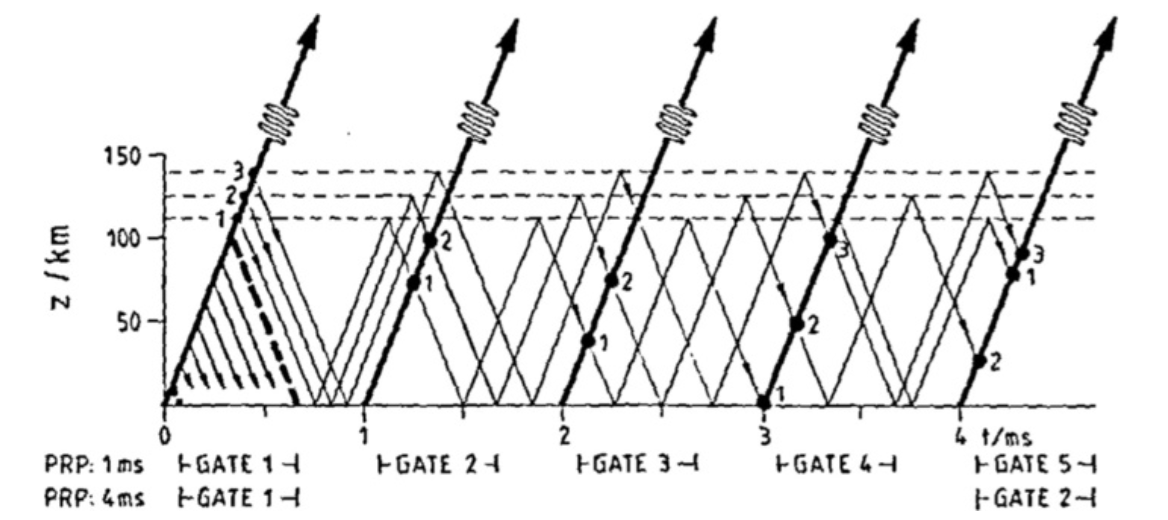
\includegraphics[width=0.8\textwidth]{images/maxPRF}	
	\caption{Range-time diagram \citep[c.f.][Fig. 5]{reid2015mf} }
\end{figure}


\subsection{Main Principle of spaced antenna techniques}
Spaced Antenna (SA) techniques are usually used for investigating and observing ionospheric dynamics and to measure the "apparent motion of ground diffraction pattern across the observing region" \citep{reid2015mf}.\\
In a default operational configuration the transmitting antenna is located close to minimum three non-collinear receiving antennas to receive partial reflections from the D-region. The antennas usually work in a bi-static mode, which means there are separate antennas for transmitting and receiving. But it is also common that the same antennas are used for both transmitting and receiving, e.g. as illustrated in fig. \ref{fig:SAconfing}, where in this particular case each antenna has its own receiver.

\begin{figure}
	\centering
	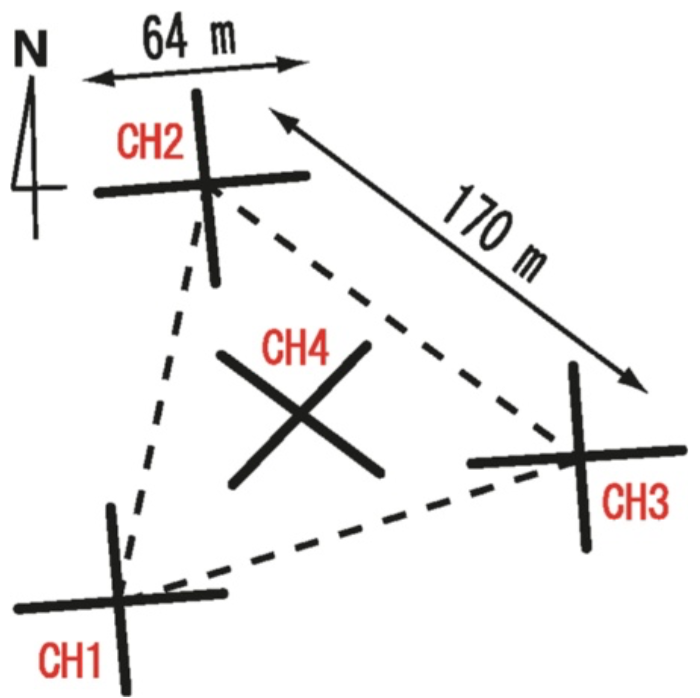
\includegraphics[width=0.5\textwidth]{images/SA_config}
	\caption{typical SA configuration at 2.43MHz (Poker Flat MF radar) \citep[c.f][Fig. 2]{reid2015mf} }
	\label{fig:SAconfing}
\end{figure}

To analyse the received signals at the three receiver antennas usually a simple correlation analysis is exerted to determine the diffraction pattern motion of the partial reflections from the D-region. In the typical case one uses coherent receivers and only the amplitude information for the analysis.

One of the advantages of this particular technique is the wide angular polar diagram one obtains when the backscatter angle is wide, thus resulting in a wide effective beam.\\
Still, this technique has some disadvantages, as for example a large area is required to place the antennas. And also the antennas need a large dynamic range for the returned echo power, which is a problem for especially older systems, since those may not have sufficient digitization capabilities \citep{reid2015mf}.

\subsection{Apparent and true velocity}
The apparent velocity is the motion of the ground diffraction pattern over the spaced antenna location, and is calculated using the time delays of the cross-correlation function which is determined between the pairs of antennas. The apparent vertical velocity is measured utilizing the phase of the complex autocorrelation function. \\
Using that simple correlation analysis, basically being a similar fades analysis, one does not take into account random changes in the pattern motion and the anisotropy in the pattern, as the pattern moves. This results in an overestimation of the \textit{true velocity} magnitude. \\
Thus, the true velocity describes the velocity, that takes into account the just stated phenomena, basically a corrected version of the apparent velocity.
\todo{include Fig 12 from REID paper}


\subsection{Deficiency of full correlation analysis for MF/HF}

The major flaw of the Full Correlation Analysis (FCA) is the very high underestimation of wind magnitude of 15\% to 40\% for an ideally configured system. According to Reid \citep{reid2015mf} this is an unacceptably high number for studies of wind dynamics. This bias is highly height dependant for MF and HF SA radars, but the reason for this is not fully understood, though the assumption of insufficient sampling of the ground diffraction pattern has been made \citep{reid2015mf}.






